\documentclass{article}

\usepackage{neurips_2026}

\usepackage[utf8]{inputenc} % allow utf-8 input
\usepackage[T1]{fontenc}    % use 8-bit T1 fonts
\usepackage{hyperref}       % hyperlinks
\usepackage{url}            % simple URL typesetting
\usepackage{booktabs}       % professional-quality tables
\usepackage{amsfonts}       % blackboard math symbols
\usepackage{nicefrac}       % compact symbols for 1/2, etc.
\usepackage{microtype}      % microtypography
\usepackage{xcolor}         % colors

\usepackage{tabularx}
\usepackage{times}
\usepackage{soul}
\usepackage{caption}
\usepackage{graphicx}
\usepackage{subcaption}
\usepackage{amsmath}
\usepackage{amsthm}
\usepackage{amssymb}
\usepackage{algorithm}
\usepackage{algorithmicx}
\usepackage[noend]{algpseudocode}
\usepackage{multicol}
\usepackage{wrapfig}
\usepackage{multirow}
\usepackage{comment}
\usepackage{tikz}
\usetikzlibrary{positioning,shapes.geometric,shapes.misc}


\newtheorem{definition}{Definition}
\newtheorem{theorem}{Theorem}
\newtheorem{lemma}{Lemma}
\newtheorem{example}{Example}

\newcommand{\pr}[1]{\mathbb{P}\!\left( #1 \right)}

% Macros for the NeurIPS 2026 LCN paper

% Calligraphic shortcuts
\newcommand{\cL}{\mathcal{L}}
\newcommand{\cS}{\mathcal{S}}
\newcommand{\cF}{\mathcal{F}}
\newcommand{\cG}{\mathcal{G}}
\newcommand{\cN}{\mathcal{N}}
\newcommand{\cA}{\mathcal{A}}
\newcommand{\cK}{\mathcal{K}}
\newcommand{\cT}{\mathcal{T}}
\newcommand{\cO}{\mathcal{O}}

% Bold shortcuts
\newcommand{\bX}{\mathbf{X}}
\newcommand{\bY}{\mathbf{Y}}
\newcommand{\bZ}{\mathbf{Z}}
\newcommand{\bx}{\mathbf{x}}
\newcommand{\by}{\mathbf{y}}
\newcommand{\bz}{\mathbf{z}}
\newcommand{\bl}{\mathbf{l}}
\newcommand{\bu}{\mathbf{u}}
\newcommand{\bq}{\mathbf{q}}
\newcommand{\bp}{\mathbf{p}}
\newcommand{\bm}{\mathbf{m}}
\newcommand{\bo}{\mathbf{o}}

% Operators
\newcommand{\pa}{\mathrm{pa}}
\newcommand{\bd}{\mathrm{bd}}
\newcommand{\scope}{\mathrm{scope}}
\newcommand{\ext}{\mathrm{ext}}
\newcommand{\prune}{\mathrm{prune}}
\newcommand{\VE}{\mathrm{VE}}


\title{New Advances in Approximate Inference for\\Logical Credal Networks}

\author{%
  David S.~Hippocampus\thanks{Use footnote for providing further information
    about author (webpage, alternative address)---\emph{not} for acknowledging
    funding agencies.} \\
  Department of Computer Science\\
  Cranberry-Lemon University\\
  Pittsburgh, PA 15213 \\
  \texttt{hippo@cs.cranberry-lemon.edu} \\
}


\begin{document}

\maketitle


\begin{abstract}
Logical Credal Networks (LCNs) are an expressive probabilistic logic that combines propositional logic formulas with imprecise probability bounds to specify sets of probability distributions. While LCNs are highly expressive---allowing cyclic dependencies and few syntactic restrictions---inference remains challenging: existing exact methods scale exponentially with the number of propositions, and the only available approximate scheme relies on a single message-passing algorithm (ARIEL). In this paper, we exploit the chain graph structure underlying LCNs to decompose inference into local credal network problems, and we introduce three new approximate inference algorithms that operate on this decomposition: (1)~\emph{Credal Variable Elimination} (CVE) with $\varepsilon$-pruning, an FPTAS that produces outer bounds with controllable accuracy; (2)~\emph{Interval Belief Propagation} (IBP), a message-passing scheme that propagates interval-vector messages and produces outer bounds; and (3)~\emph{ApproxLP}, a coordinate descent method that produces complementary inner bounds. We evaluate these algorithms on a suite of randomly generated and benchmark LCN instances, demonstrating significant speedups over exact inference while maintaining high-quality probability bounds.
\end{abstract}


%% ================================================================
\section{Introduction}
\label{sec-intro}
%% ================================================================

Combining logical and probabilistic reasoning is a long-standing goal of artificial intelligence. Frameworks such as Markov Logic Networks~\cite{richardson2006markov}, ProbLog~\cite{deraedt2007problog}, and Probabilistic Soft Logic~\cite{bach2017hinge} allow encoding domain knowledge through logical rules augmented with uncertainty. However, most of these formalisms require precise probability values and make strong structural assumptions (e.g., acyclicity).

\emph{Logical Credal Networks} (LCNs)~\cite{marinescu2022neurips} offer a more general approach: they allow \emph{imprecise} probability specifications in the form of bounds $\alpha \leq P(\phi|\varphi) \leq \beta$ on arbitrary propositional logic formulas, without requiring acyclicity. An LCN defines a \emph{credal set}---a convex set of probability distributions consistent with the given constraints---and inference amounts to computing tight lower and upper bounds on posterior probabilities of query formulas.

Previous work on LCNs has introduced exact inference via constrained optimization~\cite{marinescu2022neurips}, approximate message-passing via the ARIEL scheme~\cite{marinescu2023lcn}, and abductive reasoning~\cite{marinescu2024neurips}. The factorization properties of LCNs through chain graphs have also been studied~\cite{cozman2024ijar}. However, the exact approach scales exponentially with the number of propositions, and ARIEL is the only available approximate algorithm, limiting the practical applicability of LCNs to small instances.

In this paper, we make the following contributions:
\begin{enumerate}
    \item We show how the chain graph structure of an LCN can be exploited to decompose the global inference problem into local credal network inference tasks, bridging LCNs and the well-studied credal network formalism.
    \item We introduce three new approximate inference algorithms that operate on this decomposition:
    \begin{itemize}
        \item \textbf{Credal Variable Elimination (CVE)} with $\varepsilon$-pruning: a bucket elimination scheme that produces \emph{outer bounds} and constitutes a fully polynomial-time approximation scheme (FPTAS) for bounded treewidth networks.
        \item \textbf{Interval Belief Propagation (IBP)}: a message-passing algorithm that propagates interval-vector messages on the factor graph and produces \emph{outer bounds}, with native support for multi-valued variables.
        \item \textbf{ApproxLP}: a coordinate descent algorithm that produces complementary \emph{inner bounds} by iteratively optimizing over extreme points.
    \end{itemize}
    \item We provide an experimental evaluation on randomly generated and benchmark LCN instances, comparing accuracy and runtime of all three algorithms against exact inference.
\end{enumerate}


%% ================================================================
\section{Background}
\label{sec-background}
%% ================================================================

\subsection{Logical Credal Networks}

A Logical Credal Network (LCN) consists of a set of propositions $\cA$ and two sets of constraints $\cT_U$ and $\cT_D$. The set $\cA$ is finite with propositions $A_1, \dots, A_n$. Each proposition $A_i$ is associated with a binary indicator variable $X_i$: if $A_i$ holds in an interpretation then $X_i=1$; otherwise, $X_i=0$. Each constraint in $\cT_U$ and in $\cT_D$ is of the form:
\begin{equation}
\alpha \leq P(\phi|\varphi) \leq \beta,
\end{equation}
where $\phi$ and $\varphi$ are propositional logic formulas over $\cA$. The formula $\varphi$ can be a tautology $\top$, yielding an unconditional constraint $P(\phi)$. There is no syntactic difference between constraints in $\cT_U$ and $\cT_D$; the distinction lies in how they influence the graphical structure of the LCN (as described below).

\paragraph{Primal Graph of the LCN.} The semantics of an LCN is given by a translation to a directed graph called the \emph{primal graph}. Each proposition is a node (a \emph{proposition-node}). Each constraint $\alpha \leq P(\phi|\varphi) \leq \beta$ is processed as follows:
\begin{enumerate}
    \item A node labeled with formula $\phi$ is added (a \emph{formula-node}), and a directed edge is added from $\phi$ to each proposition in $\phi$.
    \item If the constraint is in $\cT_U$, an edge is added from each proposition in $\phi$ to node $\phi$ (creating bidirected edges).
    \item If $\varphi \neq \top$, a node labeled $\varphi$ is added, a directed edge from $\varphi$ to $\phi$ is added, and edges from each proposition in $\varphi$ to $\varphi$ are added.
\end{enumerate}

The distinction between $\cT_U$ and $\cT_D$ is that a formula in $\cT_U$ introduces bidirected (hence undirected) edges between conditioned propositions, eliminating the possibility that they are independent, while a formula in $\cT_D$ only introduces directed edges, leaving open the possibility of independence~\cite{marinescu2022neurips,cozman2024ijar}.

\begin{figure}[t]
  \centering
  \begin{subfigure}{0.4\textwidth}
    
\includegraphics[width=\textwidth]{figs/fig-lcn1-pg.png}
    \caption{Primal graph}
    \label{fig:ex1-pg}
  \end{subfigure}
  \qquad
  \begin{subfigure}{0.3\textwidth}
    
\includegraphics[scale=0.6]{figs/fig-lcn1-st.png}
    \caption{Structure}
    \label{fig:ex1-st}
  \end{subfigure}
  \caption{Primal graph and structure of the LCN from Example~\ref{ex:Smokers}.}
  \label{fig:ex1}
\end{figure}


\begin{example}\label{ex:Smokers}
    Consider the following LCN, based on the Smokers and Friends example by \cite{marinescu2022neurips}. We have propositions $C_i$, $F_i$, $S_i$ for $i\in\{1,2,3\}$. All constraints belong to $\cT_U$ (that is, $\cT_D$ is empty), with $i,j \in \{1,2,3\}$:

\[
\begin{array}{ll}
0.5 \leq P(F_i | F_j \wedge F_k) \leq 1, & i \neq j, i \neq k, j \neq k; \\
0.1 \leq P(S_i \vee S_j | F_i) \leq 0.2, & i \neq j; \\
0.03 \leq P(C_i|S_i) \leq 0.04; & \\
0.01 \leq P(C_i | \neg S_i) \leq 0.02.
\end{array}
\]

    The primal graph of this LCN is depicted in Figure~\ref{fig:ex1-pg}. Note that there are several directed cycles. The structure is depicted in Figure~\ref{fig:ex1-st}.
\end{example}


\begin{figure}[t]
  \centering
  \begin{subfigure}{0.4\textwidth}
    
\includegraphics[width=\textwidth]{figs/fig-lcn2-pg.png}
    \caption{Primal graph}
    \label{fig:ex2-pg}
  \end{subfigure}
  \qquad
  \begin{subfigure}{0.3\textwidth}
    
\includegraphics[scale=0.8]{figs/fig-lcn2-st.png}
    \caption{Structure}
    \label{fig:ex2-st}
  \end{subfigure}
  \caption{Primal graph and structure of the LCN from Example~\ref{ex:Earthquake}.}
  \label{fig:ex2}
\end{figure}


\begin{example}\label{ex:Earthquake}
   Consider another LCN based on the Earthquake example from \cite{cozman2024ijar} and defined by the following constraints:

\[
\begin{array}{ll}
0.1 \leq P(B) \leq 0.2 & \\
0.05 \leq P(E) \leq 0.1 & \\
0.8 \leq P(A|B \vee E) \leq 0.9 & \\
0.7 \leq P(\neg (C \oplus D) | A) \leq 0.8 & \\
0.01 \leq P(A) \leq 0.05 &
\end{array}
\]

    The primal graph and structure are shown in Figures~\ref{fig:ex2-pg} and \ref{fig:ex2-st}, respectively.
\end{example}


\paragraph{Structure of the LCN.} We introduce the \emph{structure} of the LCN, a graph extracted from the primal graph as follows:
\begin{enumerate}
    \item For each formula-node $\phi$ appearing as a conditioned formula in a constraint in $\cT_U$, place an undirected edge between any two propositions in $\phi$.
    \item For each pair of formula-nodes $\varphi$ and $\phi$ in a constraint, add a directed edge from each proposition in $\varphi$ to each proposition in $\phi$.
    \item If there is now a pair of edges $A \leftrightarrows B$ for some propositions $A, B$, replace both by an undirected edge.
    \item Remove formula-nodes and all their edges; remove duplicate edges.
\end{enumerate}

\subsection{Chain Graphs}

A \emph{graph} is defined by a tuple $\langle \cN, \mathcal{E}_D, \mathcal{E}_U \rangle$, where $\cN$ is a set of nodes, $\mathcal{E}_D$ are directed edges, and $\mathcal{E}_U$ are undirected edges. A \emph{path} from $A$ to $B$ is a sequence of distinct edges such that consecutive nodes satisfy either $D_1 \rightarrow D_2$ or $D_1 - D_2$ but never $D_2 \rightarrow D_1$. A \emph{directed cycle} is a cycle containing at least one directed edge. A graph without directed cycles is a \emph{chain graph}~\cite{frydenberg1990chain,lauritzen1989graphical}. The structures in Figures~\ref{fig:ex1-st} and~\ref{fig:ex2-st} are chain graphs.

\subsection{Factorization for Chain Graphs}
\label{sec-factorization}

Let $\cG$ be a chain graph with nodes $\cN$. The \emph{local Markov condition} (LMC) states:

\begin{definition}[LMC(C)]
    A node $A$ is independent, given its boundary $\bd(A)$, of all nodes that are not $A$ itself nor descendants of $A$ nor boundary nodes of $A$.
\end{definition}

Assuming positive probabilities, the local and global Markov conditions are equivalent and yield a \emph{factorization property}~\cite{cowell99}. Let $T_1, \dots, T_n$ be the chain components ordered so that nodes in $T_i$ can only be at the end of directed edges from earlier components. Then:
\begin{equation}\label{eq:factorization}
\pr{\bX=\bx} = \prod_{i=1}^n \pr{\cN_i=\bx_{\cN_i}\mid\bd(\cN_i)=\bx_{\bd(\cN_i)}}
\end{equation}
where $\cN_i$ is the set of nodes in the $i$th chain component, and $\bx_{\cN_i}$, $\bx_{\bd(\cN_i)}$ are the projections of $\bx$ over $\cN_i$ and $\bd(\cN_i)$. Each factor further factorizes according to an undirected graph built from the corresponding chain component and its boundary~\cite{cowell99}.


%% ================================================================
\section{From LCNs to Credal Networks}
\label{sec-lcn-to-credal}
%% ================================================================

In this section, we show how the chain graph factorization of an LCN can be exploited to convert the inference problem into a credal network inference problem. Let $\cL$ be an LCN whose structure is a chain graph; we call $\cL$ a \emph{chain graph LCN}.

\subsection{The Factorization Pipeline}

The conversion proceeds through the following steps:
\begin{enumerate}
    \item \textbf{Build the primal graph} of the LCN and extract its structure.
    \item \textbf{Simplify the structure} into a chain graph by identifying chain components and their parent sets.
    \item \textbf{Identify families}: each chain component $T_i$ together with its parents $\pa(T_i)$ forms a \emph{family} $\langle T_i, \pa(T_i) \rangle$.
    \item \textbf{Solve local subproblems}: for each family and each configuration $\bx$ of variables $\{T_i \cup \pa(T_i)\}$, solve a local linear-fractional program to obtain bounds $[lb, ub]$ on the conditional probability $P(T_i = \bx_{T_i} \mid \pa(T_i) = \bx_{\pa(T_i)})$. This is achieved via the Charnes-Cooper transformation~\cite{charnes1962programming} applied to the LCN constraints defined on the family.
    \item \textbf{Enumerate extreme points}: for each local credal set, compute the extreme points (vertices) using LRS vertex enumeration~\cite{avis1992pivoting}.
\end{enumerate}

The result is a \emph{credal network}: a DAG where each node $X_i$ is associated with a conditional credal set $\cK(X_i \mid \pa(X_i))$ specified by its extreme points. Standard credal network inference algorithms can then be applied.

\begin{algorithm}[t]
  \caption{LCN to Credal Network}
  \label{alg:lcn2credal}
    \begin{algorithmic}[1]
    \State Let $\cL$ be the input LCN
    \State Let $\cS$ be $\cL$'s structure (a chain graph)
    \State Let $\cF$ be the factorization of $\cS$: $P(\bx) = \prod_i P(T_i | \pa(T_i))$
    \ForAll{family $\langle T_i, \pa(T_i)\rangle$}
        \ForAll{configuration $\bx$ of variables $\{T_i \cup \pa(T_i)\}$}
            \State Let $S_i = \{s_1, ..., s_k\}$ be $\cL$'s constraints defined on $\{T_i \cup \pa(T_i)\}$
            \State $lb \leftarrow \min(\text{Charnes-Cooper}(\bx, S_i))$
            \State $ub \leftarrow \max(\text{Charnes-Cooper}(\bx, S_i))$
            \State Record interval $\cK_i(\bx) = [lb, ub]$
        \EndFor
        \State Enumerate extreme points of $\cK_i$ via LRS
    \EndFor
    \State \Return Credal network with extreme points $\{\ext\,\cK(X_i \mid \pa(X_i))\}$
    \end{algorithmic}
\end{algorithm}

\subsection{Factor Graph Representation}

Given the credal network, we construct a \textbf{factor graph}: a bipartite graph with variable nodes and factor nodes. Each variable $X_i$ corresponds to a variable node with cardinality $|D_i|$. Each conditional credal set $\cK(X_i \mid \pa(X_i))$ defines a factor node $f_i$ whose scope is $\{X_i\} \cup \pa(X_i)$. The factor stores the extreme points of $\cK(X_i \mid \pi)$ for all parent configurations~$\pi$.

\begin{example}[Alarm Network]\label{ex:alarm}
Consider the LCN from Example~\ref{ex:Earthquake}. After the chain graph factorization and LRS vertex enumeration, the resulting credal network has four nodes: $B$ (binary), $E$ (binary), $A$ (binary), and $CD$ (4-valued, representing the compound variable for $C$ and $D$), with DAG structure $B \to A$, $E \to A$, $A \to CD$. The factor graph is:

\begin{center}
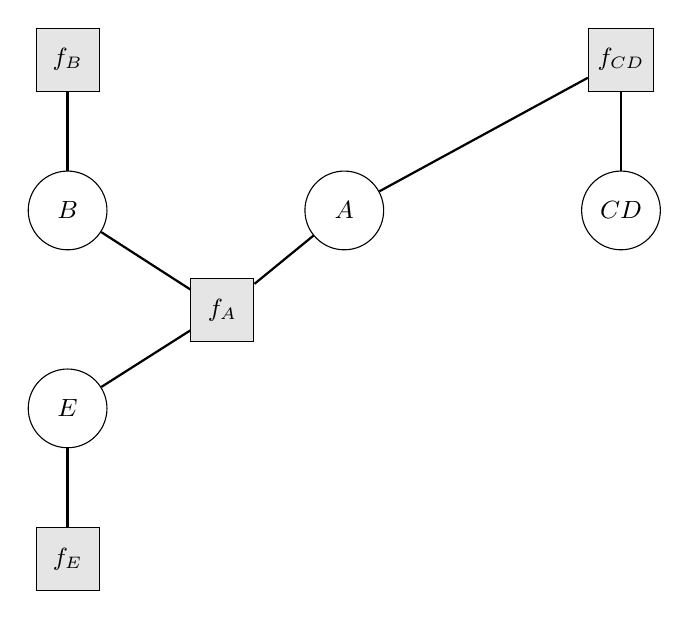
\begin{tikzpicture}[
  var/.style={circle, draw, minimum size=10mm, font=\small},
  fac/.style={rectangle, draw, fill=gray!20, minimum size=8mm, font=\small},
  edge/.style={thick},
  node distance=18mm
]
  \node[var] (B) {$B$};
  \node[var, right=25mm of B] (A) {$A$};
  \node[var, below=15mm of B] (E) {$E$};
  \node[var, right=25mm of A] (CD) {$CD$};
  \node[fac, above=10mm of B] (fB) {$f_B$};
  \node[fac, below=10mm of E] (fE) {$f_E$};
  \node[fac, below right=5mm and 12mm of B] (fA) {$f_A$};
  \node[fac, above=10mm of CD] (fCD) {$f_{CD}$};
  \draw[edge] (B) -- (fB);
  \draw[edge] (E) -- (fE);
  \draw[edge] (B) -- (fA);
  \draw[edge] (E) -- (fA);
  \draw[edge] (A) -- (fA);
  \draw[edge] (A) -- (fCD);
  \draw[edge] (CD) -- (fCD);
\end{tikzpicture}
\end{center}

\noindent The credal factors (extreme points) for each node are shown in Table~\ref{tab:credal-factors}.
\end{example}

\begin{table}[t]
\caption{Credal factors (extreme points) for the alarm network.}
\label{tab:credal-factors}
\centering
\begin{small}
\begin{tabular}{llcc}
\toprule
\textbf{Factor / Config} & \textbf{Vertex} & $P(\cdot{=}0)$ & $P(\cdot{=}1)$ \\
\midrule
$f_B$: $K(B)$ & $v_1$ & 0.80 & 0.20 \\
 & $v_2$ & 0.90 & 0.10 \\
\midrule
$f_E$: $K(E)$ & $v_1$ & 0.90 & 0.10 \\
 & $v_2$ & 0.95 & 0.05 \\
\midrule
$f_A$: $B{=}0, E{=}0$ & $v_1$ & 0.9556 & 0.0444 \\
 & $v_2$ & 1.0000 & 0.0000 \\
$f_A$: $B{=}1, E{=}0$ & $v_1$ & 0.0000 & 1.0000 \\
 & $v_2$ & 1.0000 & 0.0000 \\
$f_A$: $B{=}0, E{=}1$ & $v_1$ & 0.0000 & 1.0000 \\
 & $v_2$ & 1.0000 & 0.0000 \\
$f_A$: $B{=}1, E{=}1$ & $v_1$ & 0.0000 & 1.0000 \\
 & $v_2$ & 1.0000 & 0.0000 \\
\bottomrule
\end{tabular}
\end{small}
\end{table}


%% ================================================================
\section{Approximate Inference Algorithms}
\label{sec-algorithms}
%% ================================================================

Given the credal network obtained from the LCN factorization (Section~\ref{sec-lcn-to-credal}), we now present three approximate inference algorithms for computing marginal probability bounds. Each algorithm offers different tradeoffs between bound quality, computational cost, and bound direction (inner vs.\ outer).

\subsection{Credal Variable Elimination}
\label{sec-cve}

Credal Variable Elimination (CVE) extends classical variable elimination~\cite{dechter1999bucket} to credal networks by operating on \emph{potentials}---finite sets of non-negative functions.

\begin{definition}[Potential]
A \textbf{potential} $\phi(\bY)$ over variables $\bY$ is a finite set
of non-negative real-valued functions $\{f_1, f_2, \dots, f_m\}$ on the joint domain
of $\bY$.
\end{definition}

Three operations on potentials are central to CVE:

\paragraph{Product.}
$\phi \cdot \psi = \{f \cdot g : f \in \phi, \; g \in \psi\}$,
where $(f \cdot g)(\by, \bz) = f(\by) \cdot g(\bz)$
over the joint domain $\bY \cup \bZ$.

\paragraph{Sum-Marginal.}
$\sum_{X} \phi(\bY) = \{ \sum_{x} f(\by) : f \in \phi \}$,
producing functions over $\bY \setminus \{X\}$.

\paragraph{Pruning.}
$\prune(\phi) = \{f \in \phi : \nexists\, g \in \phi \setminus \{f\}
\text{ s.t.\ } g(\by) \geq f(\by)\; \forall\, \by\}$.
This reduces potential cardinality without affecting min/max bounds.

\paragraph{The CVE Algorithm.} CVE initializes a potential for each variable from its credal set extreme points and adds indicator potentials for evidence. It then eliminates variables one by one (in a chosen ordering), combining all potentials involving the current variable, marginalizing it out, and pruning dominated functions. The final potential over the query variable yields exact bounds after normalization.

\begin{algorithm}[t]
\caption{Credal Variable Elimination (CVE)}
\label{alg:cve}
\begin{algorithmic}[1]
\Require Extreme points $\ext\,\cK(X_i \mid \pa(X_i))$ for each node $X_i$,
         query variable $Z$, evidence $\bY = \by$
\Ensure Bounds $[\underline{P}(Z{=}z \mid \by),\; \overline{P}(Z{=}z \mid \by)]$ for each $z$
\Statex
\State $\Gamma \gets \emptyset$
\For{each variable $X_i \in \bX$}
  \State $\phi_{X_i} \gets \{p : p \in \ext\,\cK(X_i \mid \pa(X_i))\}$;
  $\Gamma \gets \Gamma \cup \{\phi_{X_i}\}$
\EndFor
\For{each evidence variable $Y_j \in \bY$}
  \State $\Gamma \gets \Gamma \cup \{\{\delta_{y_j}\}\}$
  \Comment{Indicator potential}
\EndFor
\State Compute elimination ordering $\bo$ excluding $Z$
\For{each $X_i$ in ordering $\bo$}
  \State $\Gamma_{X_i} \gets \{\phi \in \Gamma : X_i \in \scope(\phi)\}$;
  $\Gamma \gets \Gamma \setminus \Gamma_{X_i}$
  \State $\psi \gets \prod \{\phi \in \Gamma_{X_i}\}$
  \Comment{Combine potentials}
  \State $\psi' \gets \sum_{X_i} \psi$
  \Comment{Marginalize out $X_i$}
  \State $\psi'' \gets \prune(\psi')$
  \Comment{Remove dominated functions}
  \State $\Gamma \gets \Gamma \cup \{\psi''\}$
\EndFor
\State Extract and normalize bounds from remaining potentials over $Z$
\end{algorithmic}
\end{algorithm}

\paragraph{$\varepsilon$-Approximate CVE.} While exact CVE preserves tight bounds, intermediate potentials can grow exponentially. Following~\cite{maua2012anytime}, we relax the pruning criterion: a function $f$ is \emph{$\varepsilon$-dominated} by $g$ if $g(\by) \geq f(\by) - \varepsilon$ for all $\by$. Replacing exact pruning with $\varepsilon$-pruning at each step yields an approximate algorithm.

\begin{definition}[$\varepsilon$-Pruning]
$\prune_\varepsilon(\phi) = \{f \in \phi : \nexists\, g \in \phi \setminus \{f\}
\text{ s.t.\ } g(\by) \geq f(\by) - \varepsilon\; \forall\, \by\}$.
\end{definition}

Since $\varepsilon$-pruning only removes functions, the approximate bounds are always valid \emph{outer} approximations: $\underline{P}_\varepsilon \leq \underline{P}$ and $\overline{P}_\varepsilon \geq \overline{P}$.

\begin{theorem}[FPTAS~\cite{maua2012anytime}]
For credal networks of bounded treewidth $w^*$ and bounded variable cardinality $k$,
$\varepsilon$-approximate CVE runs in time polynomial in the input size and $1/\varepsilon$, producing bounds within $O(\varepsilon)$ of the exact bounds.
\end{theorem}

\paragraph{Complexity.} The cost of exact CVE is $O(n \cdot C \cdot k^{w^*})$ where $C$ is the maximum potential cardinality (which can be exponential). With $\varepsilon$-pruning, $C$ is bounded polynomially in $1/\varepsilon$.


\subsection{Interval Belief Propagation}
\label{sec-ibp}

Interval Belief Propagation (IBP) is an iterative message-passing algorithm for approximate marginal inference that propagates \emph{interval messages} on the factor graph. Unlike L2U and GL2U~\cite{ide2014credal} which are restricted to binary variables, IBP operates natively on multi-valued variables.

\begin{definition}[Interval Message]
For a variable $X$ with $k$ states, an \textbf{interval message} is a pair of vectors $(\bl, \bu) \in \mathbb{R}^k \times \mathbb{R}^k$ where $0 \leq l_x \leq u_x \leq 1$ for each state $x$. Messages are of two types: variable-to-factor $\mu_{v \to f}$ and factor-to-variable $\mu_{f \to v}$.
\end{definition}

All messages are initialized to the vacuous interval $([0, \dots, 0], [1, \dots, 1])$. Evidence variables have their messages fixed to indicator vectors.

\paragraph{Variable-to-Factor Updates.} Variable $v$ sends to factor $f$ the \emph{intersection} of messages from all other neighboring factors:
\begin{align*}
  l_{v \to f}(x) &= \max_{f' \in \cN(v) \setminus \{f\}} l_{f' \to v}(x), \\
  u_{v \to f}(x) &= \min_{f' \in \cN(v) \setminus \{f\}} u_{f' \to v}(x),
\end{align*}
with the constraint $u_{v \to f}(x) \geq l_{v \to f}(x)$ enforced.

\paragraph{Factor-to-Variable Updates.} The message from factor $f_i$ to target variable $v$ is computed by scanning over all \emph{vertex combinations} and \emph{corner-point combinations}.

\begin{definition}[Vertex Combination]
A vertex combination $\mathbf{vc} = (j_1, \dots, j_m)$ selects one extreme point per parent configuration of factor $f_i$, specifying a complete conditional distribution $P_{\mathbf{vc}}(X_i \mid \pi_k)$ for every parent configuration $\pi_k$. The total number is $\prod_{k=1}^{m} n_{\pi_k}$.
\end{definition}

\begin{definition}[Corner-Point Combination]
A corner-point combination $\mathbf{cc} = (c_1, \dots, c_{|\cO|})$ with $c_j \in \{0,1\}$ selects either the lower or upper bound vector for each ``other'' variable $w_j \in \cO = \scope(f_i) \setminus \{v\}$. The total number is $2^{|\cO|}$.
\end{definition}

For each $(\mathbf{vc}, \mathbf{cc})$ pair, the unnormalized marginal over $v$ is computed as:

\noindent\textbf{Case 1} ($v = X_i$, target is child):
\begin{equation}\label{eq:ibp-case1}
  m(v{=}x) = \sum_{\pi} P_{\mathbf{vc}}(X_i{=}x \mid \pi)
  \cdot \prod_{w \in \pa(X_i) \cap \cO} \bq_w(\pi_w).
\end{equation}

\noindent\textbf{Case 2} ($v \in \pa(X_i)$, target is parent):
\begin{equation}\label{eq:ibp-case2}
  m(v{=}x) = \sum_{\pi : \pi_v = x}
  \Bigl(\sum_{x_i} P_{\mathbf{vc}}(X_i{=}x_i \mid \pi) \cdot \bq_{X_i}(x_i)\Bigr)
  \cdot \prod_{w \in \pa \setminus \{v\}} \bq_w(\pi_w).
\end{equation}

After normalization, the factor-to-variable message takes component-wise min/max over all pairs:
$l_{f \to v}(x) = \min_{\mathbf{vc},\mathbf{cc}} p(x)$, \;
$u_{f \to v}(x) = \max_{\mathbf{vc},\mathbf{cc}} p(x)$.

\paragraph{Marginal Extraction.} After convergence, bounds for query variable $Z$ are:
$\underline{P}(z) = \max_{f \in \cN(Z)} l_{f \to Z}(z)$, \;
$\overline{P}(z) = \min_{f \in \cN(Z)} u_{f \to Z}(z)$.

\paragraph{Properties.} IBP produces \emph{outer bounds}. On polytree-structured networks, it converges to exact bounds. On loopy graphs, convergence to a fixed point is empirically observed but not guaranteed. The complexity per iteration is $O(N_f \cdot V_{\max} \cdot 2^{S_{\max}} \cdot k^{S_{\max}})$, where $N_f$ is the number of factors, $V_{\max}$ the maximum vertex combinations per factor, $S_{\max}$ the maximum scope size, and $k$ the maximum domain size.


\subsection{ApproxLP: Coordinate Descent}
\label{sec-approxlp}

ApproxLP reformulates credal marginal inference as a multilinear program and solves it via coordinate descent~\cite{antonucci2013approximate,antonucci2015finite}. The key insight is: if all local distributions $P(X_j \mid \pi_j)$ for $j \neq i$ are fixed to specific values, the program becomes \emph{linear} in $P(X_i \mid \pi_i)$. Since the optimum of a linear program over a polytope is attained at a vertex, and we have the extreme points from LRS enumeration, the optimization reduces to trying each extreme point and selecting the best one---no LP solver is needed.

\begin{algorithm}[t]
\caption{ApproxLP: Coordinate Descent over Extreme Points}
\label{alg:approxlp}
\begin{algorithmic}[1]
\Require Credal factors with extreme points, query $Z$, evidence $\bY{=}\by$,
         max iterations $T$, sense $\in \{\min, \max\}$
\Ensure Bound on $P(Z{=}z \mid \bY{=}\by)$
\Statex
\Comment{\textsc{Initialization}}
\For{each variable $X_i$, each parent config $\pi$}
  \State $P(X_i \mid \pi) \gets \text{center}(\ext\,\cK(X_i \mid \pi))$
  \Comment{Average of extreme points}
\EndFor
\State $p^* \gets \VE(\{P(X_i \mid \pi)\},\, Z,\, \by)$
\Comment{Standard VE with fixed distributions}
\Statex
\Comment{\textsc{Coordinate Descent}}
\For{$t = 1, \dots, T$}
  \State $\mathit{improved} \gets \mathsf{false}$
  \For{each variable $X_i$, each parent config $\pi$}
      \State $P_{\mathrm{best}} \gets P(X_i \mid \pi)$
      \For{each vertex $v \in \ext\,\cK(X_i \mid \pi)$}
        \State $P(X_i \mid \pi) \gets v$;
        $p_v \gets \VE(\{P(X_j \mid \pi_j)\},\, Z,\, \by)$
        \If{$\mathrm{sense}{=}\min$ and $p_v(z) < p^*(z)$, \textbf{or} $\mathrm{sense}{=}\max$ and $p_v(z) > p^*(z)$}
          \State $p^* \gets p_v$, \; $P_{\mathrm{best}} \gets v$, \; $\mathit{improved} \gets \mathsf{true}$
        \EndIf
      \EndFor
      \State $P(X_i \mid \pi) \gets P_{\mathrm{best}}$
  \EndFor
  \If{$\neg\,\mathit{improved}$} \textbf{break} \EndIf
\EndFor
\State \Return $p^*(z)$
\end{algorithmic}
\end{algorithm}

The algorithm is run twice---with $\text{sense} = \min$ and $\text{sense} = \max$---to obtain both bounds. Each VE evaluation operates on a \emph{precise} Bayesian network (single distributions, no sets of functions), which is orders of magnitude faster than credal VE.

\paragraph{Properties.} ApproxLP produces \emph{inner bounds}: $\underline{P}_{\text{true}} \leq \underline{P}_{\text{ApproxLP}}$ and $\overline{P}_{\text{ApproxLP}} \leq \overline{P}_{\text{true}}$, because coordinate descent explores a subset of feasible extreme point combinations. Convergence is monotonic and guaranteed in finite steps, though the algorithm may reach local optima. In practice, convergence occurs in 2--5 iterations. The total complexity is $O(T \cdot V_{\text{total}} \cdot n \cdot k^{w^*})$, where $V_{\text{total}}$ is the total number of extreme points across all credal sets.

\paragraph{Complementarity with IBP.} ApproxLP's inner bounds and IBP's outer bounds are complementary: together they bracket the true probability interval from both sides. If the inner and outer bounds coincide, the exact bounds have been found.


%% ================================================================
\section{Experiments}
\label{sec-experiments}
%% ================================================================

We evaluate the three proposed algorithms on a suite of LCN instances, comparing their accuracy and runtime against exact inference.

\subsection{Setup}

\paragraph{Benchmarks.} We use LCN instances from two sources: (1)~hand-crafted benchmarks including the \texttt{alarm}, \texttt{asia}, and \texttt{cancer} networks; and (2)~randomly generated LCNs with varying graph topologies (chains, DAGs, polytrees) and sizes (5--50 propositions), produced by the LCN random generator.

\paragraph{Metrics.} For each query, we report the lower and upper bounds $[\underline{P}, \overline{P}]$ and the \emph{interval width} $\overline{P} - \underline{P}$. We compare against the exact bounds obtained by the full optimization-based solver. We also report wall-clock runtime in seconds.

\paragraph{Implementation.} All algorithms are implemented in Python using the LCN package. CVE and IBP use Pyomo with the IPOPT solver for the local LP subproblems in the factorization step. Experiments are run on [hardware specification placeholder].

\subsection{Accuracy Comparison}

\begin{table}[t]
\caption{Comparison of approximate bounds against exact inference on the alarm network.}
\label{tab:accuracy}
\centering
\begin{small}
\begin{tabular}{llcccc}
\toprule
\textbf{Query} & \textbf{Method} & $\underline{P}$ & $\overline{P}$ & Width & Time (s) \\
\midrule
\multirow{4}{*}{$P(B{=}1)$}
 & Exact & 0.1000 & 0.2000 & 0.1000 & --- \\
 & CVE ($\varepsilon{=}0$) & 0.1000 & 0.2000 & 0.1000 & --- \\
 & IBP & 0.1000 & 0.2000 & 0.1000 & --- \\
 & ApproxLP & 0.1000 & 0.2000 & 0.1000 & --- \\
\midrule
\multirow{4}{*}{$P(A{=}1 \mid B{=}0, E{=}0)$}
 & Exact & 0.0000 & 0.0444 & 0.0444 & --- \\
 & CVE ($\varepsilon{=}0$) & 0.0000 & 0.0444 & 0.0444 & --- \\
 & IBP & 0.0000 & 0.0444 & 0.0444 & --- \\
 & ApproxLP & 0.0000 & 0.0444 & 0.0444 & --- \\
\bottomrule
\end{tabular}
\end{small}
\end{table}

Table~\ref{tab:accuracy} shows results on the alarm network. All three algorithms recover the exact bounds on this small polytree-structured instance.

% TODO: Add results on larger randomly generated instances
% TODO: Add results showing the effect of epsilon on CVE accuracy
% TODO: Add results showing IBP convergence behavior

\subsection{Scalability}

\begin{table}[t]
\caption{Runtime comparison (seconds) as the number of propositions increases. [Placeholder]}
\label{tab:scalability}
\centering
\begin{small}
\begin{tabular}{lcccc}
\toprule
\textbf{Propositions} & \textbf{Exact} & \textbf{CVE ($\varepsilon{=}0.01$)} & \textbf{IBP} & \textbf{ApproxLP} \\
\midrule
10  & --- & --- & --- & --- \\
20  & --- & --- & --- & --- \\
30  & --- & --- & --- & --- \\
50  & --- & --- & --- & --- \\
\bottomrule
\end{tabular}
\end{small}
\end{table}

% TODO: Fill in experimental results

\subsection{Algorithm Comparison}

Table~\ref{tab:comparison} summarizes the key properties of each algorithm.

\begin{table}[t]
\caption{Summary of algorithm properties.}
\label{tab:comparison}
\centering
\begin{small}
\begin{tabular}{lccccc}
\toprule
\textbf{Property} & \textbf{Exact VE} & \textbf{CVE ($\varepsilon$)} & \textbf{IBP} & \textbf{ApproxLP} \\
\midrule
Exact & Yes & No & No & No \\
Bound type & Tight & Outer & Outer & Inner \\
All marginals & No & No & Yes & No \\
Multi-valued & Yes & Yes & Yes & Yes \\
Convergence & --- & FPTAS & Empirical & Monotonic \\
\bottomrule
\end{tabular}
\end{small}
\end{table}

The three algorithms offer complementary strengths. CVE with $\varepsilon$-pruning provides theoretical guarantees (FPTAS) with controllable accuracy. IBP computes bounds for all variables simultaneously through message passing. ApproxLP is the fastest method, producing inner bounds that complement the outer bounds of CVE and IBP. When ApproxLP's inner bounds and IBP's outer bounds coincide, the exact bounds have been identified without running exact inference.


%% ================================================================
\section{Related Work}
\label{sec-related}
%% ================================================================

\paragraph{Credal networks.} Credal networks~\cite{cozman2000credal} extend Bayesian networks by replacing precise conditional distributions with convex sets of distributions (credal sets). Exact inference in credal networks is NP-hard even for polytrees~\cite{maua2012anytime}. Approximate algorithms include the 2U and L2U schemes~\cite{ide2014credal} for binary variables, the GL2U extension~\cite{ide2014credal}, and the ApproxLP method~\cite{antonucci2013approximate,antonucci2015finite}. Our work adapts and extends these algorithms to operate on the credal networks derived from LCN factorization, with native support for multi-valued variables.

\paragraph{Probabilistic logic.} ProbLog~\cite{deraedt2007problog} and DeepProbLog~\cite{manhaeve2018deepproblog} combine logic programming with precise probabilities. Markov Logic Networks~\cite{richardson2006markov} attach weights to first-order logic formulas. Probabilistic Soft Logic~\cite{bach2017hinge} uses continuous truth values with hinge-loss potentials. LCNs differ from all of these by allowing \emph{imprecise} probability specifications and operating in the propositional setting with few structural restrictions.

\paragraph{LCN inference.} Previous work on LCN inference includes exact constrained optimization~\cite{marinescu2022neurips}, the ARIEL message-passing scheme~\cite{marinescu2023lcn}, and abductive (MAP) reasoning~\cite{marinescu2024neurips}. The chain graph factorization and Markov conditions were studied in~\cite{cozman2024ijar}. Our work introduces three new algorithms that exploit this factorization for scalable approximate inference.

\paragraph{Variational methods.} Mean-field variational inference has been applied to credal networks~\cite{jordan1999variational}, producing bounds by optimizing over factored approximations. Our IBP algorithm shares the iterative message-passing structure but propagates interval messages rather than point distributions.


%% ================================================================
\section{Conclusion}
\label{sec-conclusion}
%% ================================================================

We have presented three new approximate inference algorithms for Logical Credal Networks that exploit the chain graph factorization to decompose inference into local credal network problems. Credal Variable Elimination with $\varepsilon$-pruning provides an FPTAS with provable outer bounds. Interval Belief Propagation offers efficient message-passing with native multi-valued variable support. ApproxLP provides complementary inner bounds via coordinate descent. Together, these algorithms can bracket the exact probability bounds from both sides.

\paragraph{Limitations.} The factorization step requires the LCN structure to be a chain graph, which may not hold for all LCNs. The quality of IBP bounds on loopy graphs lacks formal guarantees. ApproxLP may converge to local optima. The scalability of all methods is ultimately limited by the treewidth of the underlying graph.

\paragraph{Future work.} Promising directions include extending the algorithms to handle non-chain-graph structures, developing tighter convergence bounds for IBP on loopy graphs, combining multiple random restarts with ApproxLP to escape local optima, and applying these inference methods to downstream tasks such as neuro-symbolic AI and robust decision making under imprecise probabilities.


\bibliography{ref}
\bibliographystyle{unsrt}


%%%%%%%%%%%%%%%%%%%%%%%%%%%%%%%%%%%%%%%%%%%%%%%%%%%%%%%%%%%%
\appendix

\section{Detailed Running Examples}
\label{app:examples}

We provide detailed traces of the IBP and ApproxLP algorithms on the alarm network (Example~\ref{ex:alarm}).

\subsection{IBP Trace: $P(B{=}1)$, No Evidence}

\paragraph{Iteration 1: Factor-to-Variable Messages.}

\emph{Message $f_B \to B$.}
Factor $f_B$ has scope $\{B\}$ with no parents ($\cO = \emptyset$), 2 vertex combinations, and $2^0 = 1$ corner-point combination. For each vertex:
\begin{align*}
  \mathbf{vc} = (1): \; & m = [0.80, 0.20], \; p = [0.80, 0.20]. \\
  \mathbf{vc} = (2): \; & m = [0.90, 0.10], \; p = [0.90, 0.10].
\end{align*}
Result: $\mu_{f_B \to B} = ([0.80, 0.10], [0.90, 0.20])$.

\emph{Message $f_E \to E$.} Analogously: $\mu_{f_E \to E} = ([0.90, 0.05], [0.95, 0.10])$.

\emph{Message $f_A \to A$.} With vacuous incoming messages ($\mu_{B \to f_A} = \mu_{E \to f_A} = ([0,0],[1,1])$), $2^4 = 16$ vertex combinations and $2^2 = 4$ corner-point combinations. Only $\mathbf{cc} = (1,1)$ produces nonzero marginals. For $\mathbf{vc} = (1,1,1,1)$:
\begin{align*}
  m(A{=}0) &= 0.9556 \cdot 1 \cdot 1 + 0 + 0 + 0 = 0.9556, \\
  m(A{=}1) &= 0.0444 + 1.0 + 1.0 + 1.0 = 3.0444, \\
  p &= [0.2389, 0.7611].
\end{align*}

\paragraph{Iteration 1: Variable-to-Factor Messages.}
After tightening: $\mu_{B \to f_A} = \mu_{f_B \to B} = ([0.80, 0.10], [0.90, 0.20])$ and $\mu_{E \to f_A} = \mu_{f_E \to E} = ([0.90, 0.05], [0.95, 0.10])$.

\paragraph{Iteration 2.} With informative messages, $f_A \to A$ computes tighter bounds. For $\mathbf{vc} = (1,1,1,1)$, $\bq_B = [0.80, 0.10]$, $\bq_E = [0.90, 0.05]$:
\begin{align*}
  m(A{=}0) &= 0.9556 \cdot 0.80 \cdot 0.90 = 0.6880, \\
  m(A{=}1) &= 0.0444 \cdot 0.80 \cdot 0.90 + 1.0 \cdot 0.10 \cdot 0.90 + 1.0 \cdot 0.80 \cdot 0.05 + 1.0 \cdot 0.10 \cdot 0.05 = 0.1670.
\end{align*}

\paragraph{Final result.} After convergence: $P(B{=}1) \in [0.10, 0.20]$, matching exact inference.

\subsection{ApproxLP Trace: $P(B{=}1)$, No Evidence}

\paragraph{Initialization.} Set distributions to credal set centers: $P(B) = [0.85, 0.15]$, $P(E) = [0.925, 0.075]$. Initial VE gives $P(B{=}1) = 0.15$.

\paragraph{Coordinate descent ($\min$).} Try $B$: $v_1 = [0.80, 0.20] \Rightarrow P(B{=}1) = 0.20$ (worse); $v_2 = [0.90, 0.10] \Rightarrow P(B{=}1) = 0.10$ (accept). Next iteration: no improvement. Result: $\underline{P}(B{=}1) = 0.10$.

\paragraph{Coordinate descent ($\max$).} Selecting $v_1 = [0.80, 0.20]$ gives $\overline{P}(B{=}1) = 0.20$.

\paragraph{Final result.} $P(B{=}1) \in [0.10, 0.20]$, matching exact inference.


%%%%%%%%%%%%%%%%%%%%%%%%%%%%%%%%%%%%%%%%%%%%%%%%%%%%%%%%%%%%

\newpage
% NeurIPS Paper Checklist
% TODO: Fill in the checklist before submission

\section*{NeurIPS Paper Checklist}

\begin{enumerate}

\item {\bf Claims}
    \item[] Question: Do the main claims made in the abstract and introduction accurately reflect the paper's contributions and scope?
    \item[] Answer: \answerYes{}

\item {\bf Limitations}
    \item[] Question: Does the paper discuss the limitations of the work performed by the authors?
    \item[] Answer: \answerYes{}

\item {\bf Theory assumptions and proofs}
    \item[] Question: For each theoretical result, does the paper provide the full set of assumptions and a complete (or complete reference to a) proof?
    \item[] Answer: \answerYes{}

\item {\bf Experimental result reproducibility}
    \item[] Question: Does the paper fully disclose all the information needed to reproduce the main experimental results of the paper to the extent that it affects the main claims and/or conclusions of the paper?
    \item[] Answer: \answerTODO{}

\item {\bf Code of ethics}
    \item[] Question: Does the research conducted in the paper conform, in every respect, with the NeurIPS Code of Ethics?
    \item[] Answer: \answerYes{}

\end{enumerate}



\end{document}
